\documentclass[twoside]{article}

\usepackage[preprint]{aistats2026}
\usepackage[round,authoryear]{natbib}
\usepackage{amsmath,amssymb,amsthm,mathtools}
\usepackage{booktabs}
\usepackage{microtype}
\usepackage{xcolor}
\usepackage{enumitem}
\usepackage{graphicx}
\setlength{\emergencystretch}{2em}

\renewcommand{\bibname}{References}
\renewcommand{\bibsection}{\subsubsection*{\bibname}}
\bibliographystyle{apalike}

\newtheorem{theorem}{Theorem}
\newtheorem{lemma}[theorem]{Lemma}
\newtheorem{proposition}[theorem]{Proposition}
\newtheorem{corollary}[theorem]{Corollary}
\newtheorem{remark}[theorem]{Remark}

\newcommand{\E}{\mathbb E}
\newcommand{\Pp}{\mathbb P}
\newcommand{\1}{\mathbf 1}
\newcommand{\cH}{\mathcal H}
\newcommand{\cG}{\mathcal G}
\newcommand{\cA}{\mathcal A}
\newcommand{\Reg}{\operatorname{Reg}}
\newcommand{\KL}{\operatorname{KL}}
\newcommand{\Var}{\operatorname{Var}}
\newcommand{\Bern}{\operatorname{Bernoulli}}

\begin{document}
\runningauthor{}

\twocolumn[
\aistatstitle{Balanced Learning from Attribution Sets}

\aistatsauthor{Pahan Dewasurendra}
\aistatsaddress{Johns Hopkins University}]

\begin{abstract}\sloppy
Attribution sets replace the source label of each positive event by a set of candidate examples. The first learning guarantees for this model lose a factor $1/\|\pi\|_2^2$, where $\pi$ is the prior over candidates. For a uniform set of size $k$, this gives a leading rate $k/\sqrt n$. Whether that dependence is intrinsic was left open. We show that it is not under stationary attribution. Our estimator attaches a negative control to every reported set. Translation balance cancels both row and column effects of the irrelevant candidates, leaving a canonical order-two statistic. If $\Sigma=\|\pi\|_2^2$, its variance is $O(1/(n\Sigma))$ and finite-class empirical risk minimization has leading regret \[ O\!\left(\sqrt{\frac{\log(|\cH|/\delta)}{n\Sigma}}\right). \] Uniform attribution therefore costs only $\sqrt{k}$ rather than $k$. The estimator is exactly unbiased, runs in $O(k)$ time per report, and requires neither the conversion rate nor population feature moments. A four-regime concentration theorem handles all overlap among reported sets through decoupling and sharp canonical U-statistic inequalities.

For uniform attribution, the rate is minimax sharp. On a stationary block instance, an exact likelihood projection gives a matching $\Omega(\sqrt{k/n})$ regret lower bound for two hypotheses and binary labels. We also extend the construction to ordinary paths when the reporter marks a source-defined target cohort. A max-flow argument produces diffuse boundary controls with the same rate. Simulations confirm exact debiasing and the predicted $\sqrt{k/n}$ scaling.
\end{abstract}

\section{INTRODUCTION}

Modern attribution systems often reveal that a conversion followed one of several clicks while hiding which click caused it. This protects a direct cross-site link, but it also removes the individual training label. \citet{applebaum2026attribution} recently formalized this problem. A learner observes iid feature vectors and one candidate set for every positive label. The true source occupies a random position governed by a known prior $\pi$. Candidate sets may overlap heavily.

The model is identifiable. The estimator of \citet{applebaum2026attribution} yields a generalization bound whose main terms scale as $1/(\Sigma\sqrt n)$, where
\begin{equation}
 \Sigma=\sum_{r}\pi_r^2.
 \label{eq:sigma}
\end{equation}
For a uniform prior on $k$ candidates, $\Sigma=1/k$ and the rate is $k/\sqrt n$. Their paper asks for matching regret lower bounds. A lower bound at that scale would mean that hiding one source among $k$ candidates reduces the useful sample size from $n$ to $n/k^2$.

We find a different answer under stationary attribution. The useful sample size is $n\Sigma$, which is $n/k$ for a uniform prior. The gap comes from a first-order fluctuation that unbiasedness alone does not remove. A positive report contains the true feature with squared prior mass $\Sigma$. The other candidates contribute a population feature mean. Subtracting that mean as a fixed nuisance correction leaves its empirical fluctuation intact and amplifies it by $1/\Sigma$. Our estimator instead takes the correction from examples outside the reported set. Its weights are chosen so that every source row and every feature column has zero off-source mass. This double balance turns the fluctuation into a degenerate order-two statistic.

\paragraph{Contributions.}
Our results apply to translated candidate sets on a finite abelian group. This includes consecutive wraparound windows and arbitrary translated offset patterns.

\begin{enumerate}[leftmargin=*,itemsep=2pt,topsep=3pt]
\item We give an exactly unbiased score that uses no conversion rate or population moment. It is a weighted sum over the $k$ candidates minus a uniform control over their complement. A global feature sum makes evaluation cost $O(k)$ per report.
\item We prove a single-log tail bound with leading scale $1/\sqrt{n\Sigma}$. The proof gives an exact Hoeffding decomposition. Decoupling and the four-parameter inequality of \citet{gine2000exponential} control the overlapping part without discarding reports.
\item For finite $\cH$, balanced empirical risk minimization attains $O(\sqrt{\log(|\cH|/\delta)/(n\Sigma)})$ in its Gaussian range. We display the complete tail outside that range.
\item For uniform attribution we prove the matching binary-label lower bound. A block-translation mechanism reduces each block to its positive count. Projection of the likelihood onto that count has exact chi-square divergence $\sum_{j=1}^k \rho^{2j}$. Le Cam's method gives $\Omega(\sqrt{k/n})$ regret even for $|\cH|=2$.
\item We remove the wraparound idealization for a reporting-cohort design on an ordinary path. A bounded avoidance coupling constructs nonnegative controls outside every candidate window. Numerical audits verify the flow identities and the synthetic experiment confirms the predicted scaling.
\end{enumerate}

Table~\ref{tab:comparison} summarizes the statistical change. The previous guarantee is more general in its treatment of nonstationary windows and infinite classes. Our result identifies the sharp rate under translation structure and supplies a matching lower bound.

\begin{table}[t]
\centering
\small
\caption{Leading finite-class regret, omitting logarithms. Here $\Sigma=\|\pi\|_2^2$. The lower row is for uniform priors and stationary mechanisms, uniformly over offset geometries.}
\label{tab:comparison}
\begin{tabular}{@{}lll@{}}
\toprule
Result & General $\pi$ & Uniform $k$ \\
\midrule
Prior upper bound & $1/(\Sigma\sqrt n)$ & $k/\sqrt n$ \\
This work & $1/\sqrt{n\Sigma}$ & $\sqrt{k/n}$ \\
This work, lower & uniform $\pi$ & $\sqrt{k/n}$ \\
\bottomrule
\end{tabular}
\end{table}

\section{RELATED WORK}

\paragraph{Attribution sets.}
\citet{applebaum2026attribution} introduce the observation model studied here. Their main technical result combines an unbiased loss estimate with sensitivity and covering arguments that remain valid when sets overlap. For finite classes, their theorem contains terms of order $\sqrt{\log|\cH|/n}/\Sigma$ and an overlap term depending on the conversion rate and $\min\{\log|\cH|,k\}$. The analysis assumes the class prior and two population feature moments, then explains how sample splitting estimates them at the same displayed resolution. They leave fast localized rates and matching regret lower bounds open. Our focus is different. Translation structure permits a local negative control that improves the global rate, removes those nuisance quantities, and yields a matching minimax theorem.

\paragraph{Learning from label proportions.}
Learning from label proportions observes a count or average label for each bag. Recent work has sharply improved its dependence on bag size. \citet{li2024optimistic} derive optimistic rates for proportion matching and debiased losses. \citet{busafekete2025nearly} give nearly optimal square-loss rates. \citet{applebaum2026optimal} introduce a centered low-variance estimator for general losses whose variance is independent of bag size. These papers study iid disjoint bags with an aggregate label. Attribution sets reveal one overlapping candidate set per positive example, but not the number of positives within that set. Our subtraction is related in spirit to LLP centering. The new difficulty is to balance a random superposition of overlapping reports in both source and feature coordinates.

\paragraph{Other aggregate observations.}
General weak-supervision frameworks include multiple-instance labels, pairwise and ranking observations, and label proportions. \citet{zhang2020aggregate} give a likelihood framework and characterize consistency up to observational equivalence. \citet{wei2023universal} construct unbiased risks for broad aggregate classification mechanisms. \citet{agarwal2024aggregating} study how to form disjoint bags for accurate and private learning. Those models do not provide the translated, overlapping positive-event channel analyzed here.

\paragraph{Canonical U-statistics.}
The dependency created by overlap is not handled by pretending reports are independent. We use tail decoupling for generalized U-statistics \citep{delapena1995decoupling}, followed by the sharp four-regime canonical inequality of \citet{gine2000exponential}. The four terms matter at extreme confidence. In the usual learning range, their Gaussian term gives the effective sample size $n\Sigma$.

\section{MODEL AND BALANCED SCORE}

Let $G$ be a finite abelian group of order $n$. The hidden sample $((X_t,Y_t):t\in G)$ is iid from a distribution on $\mathcal X\times\{0,1\}$. Let $K\subset G$ contain $k$ offsets, and let $\pi$ be a known probability mass function supported on $K$. For each $t$ with $Y_t=1$, the mechanism independently draws $R_t\sim\pi$ and publishes the anchor
\begin{equation}
 Z_t=t-R_t.
 \label{eq:anchor}
\end{equation}
The anchor identifies the ordered attribution set $(X_{Z_t+r}:r\in K)$. The learner observes all features and the multiset $\cA=\{Z_t:Y_t=1\}$, including multiplicity, but not the source of any element of $\cA$. This is the oblivious attribution model restricted to a translation action. On $G=\mathbb Z_n$, $K=\{0,\ldots,k-1\}$ gives consecutive cyclic windows.

Assume $n\ge2k$ and define
\begin{equation}
 c_\pi=\frac{1-\Sigma}{n-k}.
 \label{eq:cpi}
\end{equation}
For an observed anchor $z$, assign feature $s$ the score
\begin{equation}
 a_z(s)=\pi_{s-z}\1\{s-z\in K\}
       -c_\pi\1\{s-z\notin K\}.
 \label{eq:score}
\end{equation}
The first term is the posterior source weight under a uniform source index. The second is a negative control spread over every feature that could not have caused this report. The supports are disjoint, and
\begin{align}
 \sum_s a_z(s)&=\Sigma, & \|a_z\|_1&=2-\Sigma,\label{eq:mass}\\
 \|a_z\|_2^2&=\Sigma+\frac{(1-\Sigma)^2}{n-k}\le2\Sigma.\label{eq:energy}
\end{align}
The inequality uses $n-k\ge k$ and $\Sigma\ge1/k$.

For any measurable $g:\mathcal X\to[-1,1]$, estimate $\theta_g=\E[Yg(X)]$ by
\begin{equation}
 \widehat\theta_g=\frac1{n\Sigma}
 \sum_{z\in\cA}\sum_{s\in G}a_z(s)g(X_s).
 \label{eq:estimator}
\end{equation}
This is efficient despite the dense control. Precompute $S_g=\sum_sg(X_s)$. Each report needs
\begin{equation}
 \sum_{r\in K}\pi_r g(X_{z+r})
 -c_\pi\left(S_g-\sum_{r\in K}g(X_{z+r})\right),
 \label{eq:fastscore}
\end{equation}
which costs $O(k)$.

\begin{proposition}[Exact balance]\label{prop:unbiased}
For every $g:\mathcal X\to[-1,1]$, $\E\widehat\theta_g=\theta_g$. If $g$ is constant, then $\widehat\theta_g=g\sum_tY_t/n$ pathwise.
\end{proposition}

\begin{proof}
Let $A(t,s)=\E_R a_{t-R}(s)$. Its diagonal is $A(t,t)=\sum_r\pi_r^2=\Sigma$. By \eqref{eq:mass}, every off-diagonal row sums to zero. Translation invariance makes $A$ group-circulant, so every off-diagonal column also sums to zero. Independence across distinct sample indices now gives \[ \E\sum_{t,s}Y_t a_{t-R_t}(s)g(X_s) =n\Sigma\E[Yg(X)]. \] For constant $g$, \eqref{eq:mass} makes each published report contribute exactly $\Sigma g$.
\end{proof}

The column statement is the essential addition. Row centering alone proves unbiasedness, but leaves a first-order empirical feature fluctuation. Column centering removes it.

\section{SINGLE-LOG CONCENTRATION}

Write $\pi_\star=\max_r\pi_r$ and
\begin{align}
 \Psi_n(x)=&\sqrt{\frac{x}{n\Sigma}}+\frac{x}{n\Sigma}
 +\frac{x^{3/2}}{n\sqrt\Sigma}\notag\\
 &+\frac{(\pi_\star+1/(n-k))x^2}{n\Sigma}.
 \label{eq:psi}
\end{align}

\begin{theorem}[Balanced concentration]\label{thm:concentration}
There are universal constants $C,c>0$ such that, for every fixed $g:\mathcal X\to[-1,1]$ and every $x\ge1$,
\begin{equation}
 \Pp\left(|\widehat\theta_g-\theta_g|>C\Psi_n(x)\right)
 \le C e^{-x/C}.
 \label{eq:tail}
\end{equation}
In particular, $\Var(\widehat\theta_g)\le C/(n\Sigma)$. The first term in \eqref{eq:psi} dominates if
\begin{equation}
 x\le c\min\left\{n\Sigma,\sqrt n,
 \left(\frac{n\Sigma}{(\pi_\star+1/(n-k))^2}\right)^{1/3}\right\}.
 \label{eq:range}
\end{equation}
\end{theorem}

We give the proof spine here and all parameter checks in Supplementary Sections B--D. Draw $R_t\sim\pi$ even when $Y_t=0$. Put $\mu=\E g(X)$, $p=\E Y$, and $W(t,s)=\E_Ra_{t-R}(s)$ for $s\ne t$. For $s\ne t$, define
\begin{equation}
 h_{ts}=\{Y_ta_{t-R_t}(s)-pW(t,s)\}\{g(X_s)-\mu\}.
 \label{eq:kernel}
\end{equation}
This kernel is canonical in both arguments. Exact row and column balance give the identity
\begin{align}
 n\Sigma(\widehat\theta_g-\theta_g)
 &=\sum_tL_t+\sum_t\sum_{s\ne t}h_{ts},\label{eq:hoeffding}\\
 L_t&=Y_t[\pi_{R_t}\{g(X_t)-\mu\}+\mu\Sigma]-\Sigma\theta_g.
 \label{eq:linear}
\end{align}
The $L_t$ are independent and satisfy $\sum_t\Var(L_t)\le Cn\Sigma$.

For the canonical sum, the four parameters of \citet[Theorem 3.3]{gine2000exponential} obey
\begin{equation}
 C_2^2\lesssim n\Sigma,\quad B_2^2\lesssim\Sigma,
 \quad D_2\lesssim1,\quad A_2\lesssim\pi_\star+\frac1{n-k}.
 \label{eq:fourparams}
\end{equation}
Energy \eqref{eq:energy} gives the first two bounds. For $D_2$, fixing a displacement produces a matrix with absolute row and column sums at most two, so Schur's test applies. The last bound follows from \eqref{eq:score}. Tail decoupling \citep{delapena1995decoupling}, the canonical inequality, and Bernstein's inequality for \eqref{eq:linear} prove \eqref{eq:tail}. The powers $x^{3/2}$ and $x^2$ are the genuine non-Gaussian regimes of bounded canonical statistics, not a union-bound artifact.

\section{LEARNING GUARANTEE}

Let $\ell(h(x),y)\in[0,1]$ be any loss with binary $y$. Write
\begin{equation}
 \ell(h(X),Y)=f_h(X)+Yg_h(X),
 \label{eq:lossdecomp}
\end{equation}
where $f_h(X)=\ell(h(X),0)$ and $g_h(X)=\ell(h(X),1)-\ell(h(X),0)$. Define
\begin{equation}
 \widehat L(h)=\frac1n\sum_s f_h(X_s)+\widehat\theta_{g_h},
 \qquad \widehat h\in\arg\min_{h\in\cH}\widehat L(h).
 \label{eq:erm}
\end{equation}

\begin{corollary}[Finite-class ERM]\label{cor:erm}
Let $\cH$ be finite and set $x=C\log(C|\cH|/\delta)$. With probability at least $1-\delta$,
\begin{equation}
 \Reg(\widehat h)\le C\Psi_n(x).
 \label{eq:ermfull}
\end{equation}
If \eqref{eq:range} holds, this becomes
\begin{equation}
 \Reg(\widehat h)\le
 C\sqrt{\frac{\log(C|\cH|/\delta)}{n\Sigma}}.
 \label{eq:ermsimple}
\end{equation}
For uniform $\pi$, the complete bound is
\begin{equation}
 C\left[\sqrt{\frac{kx}{n}}+\frac{kx}{n}
 +\frac{\sqrt{k}x^{3/2}}n+\frac{x^2}n\right].
 \label{eq:uniformfull}
\end{equation}
\end{corollary}

\begin{proof}
Apply Theorem~\ref{thm:concentration} to every $g_h$. Hoeffding's inequality controls the ordinary feature means, and its term is no larger than the first term of \eqref{eq:psi}. A union bound and the standard ERM comparison complete the proof.
\end{proof}

The guarantee is agnostic and holds for any bounded binary loss. Unlike a position-wise inverse correction, its dependence on $\pi$ is through $1/\sqrt\Sigma$. It also has no explicit conversion-rate term. Rare conversions can yield a smaller variance than our worst-case statement, but no lower bound on their frequency is required for validity.

\section{MATCHING BINARY LOWER BOUND}

Our lower bound uses translated blocks. This geometry isolates the information loss and permits an exact divergence calculation.

\begin{theorem}[Minimax sharpness]\label{thm:lower}
There are universal constants $c,C>0$ with the following property. Let $n=mk$, $n\ge Ck$, and let $\pi$ be uniform on $k$ offsets. There is a stationary translation mechanism and a two-element class under zero-one loss such that every learner satisfies
\begin{equation}
 \sup_D\E_D\Reg(\widehat h)\ge c\sqrt{\frac{k}{n}}
 =\frac{c}{\sqrt{n\Sigma}}.
 \label{eq:reglower}
\end{equation}
The supremum is over iid binary-label distributions and the learner observes every feature and every attribution report.
\end{theorem}

\begin{proof}
Take $G=\mathbb Z_m\times\mathbb Z_k$ and $K=\{0\}\times\mathbb Z_k$. Every candidate set is one block. Its reported anchor gives an independent uniform rotation, so conditional on the positive count $M_b$ in block $b$, all anchors contain no further parameter information.

Let $X_i$ be iid Rademacher and $Y_i\mid X_i\sim\Bern(1/2+\epsilon X_i)$. At $\epsilon=0$, the normalized functions $\phi_i=2(Y_i-1/2)$ form a product Walsh basis. If $|S|=j$, conditioning on $M_b$ is permutation symmetrization and
\begin{equation}
 \left\|\E[\phi_S\mid M_b]\right\|_2^2={k\choose j}^{-1}.
 \label{eq:projection}
\end{equation}
The likelihood ratio is $\prod_i(1+2\epsilon X_i\phi_i)$. After projection onto $M_b$, averaging its squared centered value over the observed $X_i$ kills cross-subset terms. Equation \eqref{eq:projection} cancels the number of subsets, giving the exact identity
\begin{equation}
 \E_X\chi^2(P_\epsilon(M_b\mid X),P_0(M_b))
 =\sum_{j=1}^k(4\epsilon^2)^j.
 \label{eq:chisquare}
\end{equation}
For $4\epsilon^2\le1/2$, this is at most $8\epsilon^2$. KL is bounded by chi-square and adds over the $m$ blocks. Choosing $\epsilon=c_0\sqrt{k/n}$ makes the KL between parameters $\epsilon$ and $0$ a small constant. Using the symmetric pair $\epsilon$ and $-\epsilon$ changes only constants.

Finally take $h_+(x)=\1\{x=1\}$ and $h_-(x)=\1\{x=-1\}$. Their risks under parameter $\epsilon$ are $1/2-\epsilon$ and $1/2+\epsilon$, and the optimum swaps under $-\epsilon$. Le Cam's two-point lemma gives \eqref{eq:reglower}.
\end{proof}

The mechanism is stationary but uses a subgroup offset pattern rather than one fixed consecutive-window geometry. The theorem therefore establishes the optimal rate uniformly over translated attribution mechanisms. It does not claim that every particular $K$ has the same lower bound. This distinction is useful because the upper theorem holds for every $K$.

\section{PATH EXTENSION AND EXPERIMENT}

\paragraph{Ordinary paths.}
Translation made the negative control explicit. A related construction works without wraparound when the reporter identifies a target cohort before hiding individual sources. Retain $k-1$ iid context features on each side of $n_0$ target examples. Only reports generated by target sources receive the cohort flag. For window $A_z$ define its local posterior score $q_z(s)=\pi_{s-z}\1\{s\in A_z\}$. Supplementary Section F proves the following.

\begin{proposition}[Balanced path controls]\label{prop:path}
If $n_0\ge4k$, there are nonnegative weights $b_z(s)$ supported outside $A_z$ such that $a_z=q_z-b_z$ is exactly row and column balanced and
\begin{equation}
 \|a_z\|_1\le2,\qquad \|a_z\|_2^2\le\frac32\Sigma,
 \qquad \max_sb_z(s)\le\frac2{n_0}.
 \label{eq:pathenergy}
\end{equation}
They depend only on geometry and $\pi$ and can be found by max flow. Replacing \eqref{eq:score} by these weights gives Proposition~\ref{prop:unbiased}, Theorem~\ref{thm:concentration}, and Corollary~\ref{cor:erm} with $n_0$ in place of $n$ and changed universal constants.
\end{proposition}

The reporter-side cohort flag is important. It is fixed before attribution and never reveals the source within a set. The proposition does not assert that source-defined cohorts can be recovered after an unflagged path log has been released. Since $n_0\ge4k$, the $2(k-1)$ context examples increase the retained feature count by less than one half. Thus the stated rate is unchanged, up to a universal constant, when expressed in the total retained sample size.

\paragraph{Synthetic audit.}
We test the stationary estimator on Rademacher scores with $\Pp(g=1)=0.65$, $\Pp(Y=1\mid g=1)=0.7$, and $\Pp(Y=1\mid g=-1)=0.2$. Thus $\theta_g=0.385$ and the feature mean is nonzero. We use uniform consecutive cyclic windows, $1{,}500$ repetitions per configuration, and no fitted parameters. Figure~\ref{fig:scaling} shows the RMSE and its predicted normalization. Across $n\in\{256,512,1024,2048\}$ and $k\in\{2,4,8,16,32,64\}$, $\mathrm{RMSE}\sqrt{n/k}$ stays between $0.55$ and $0.71$.

\begin{figure}[t]
\centering
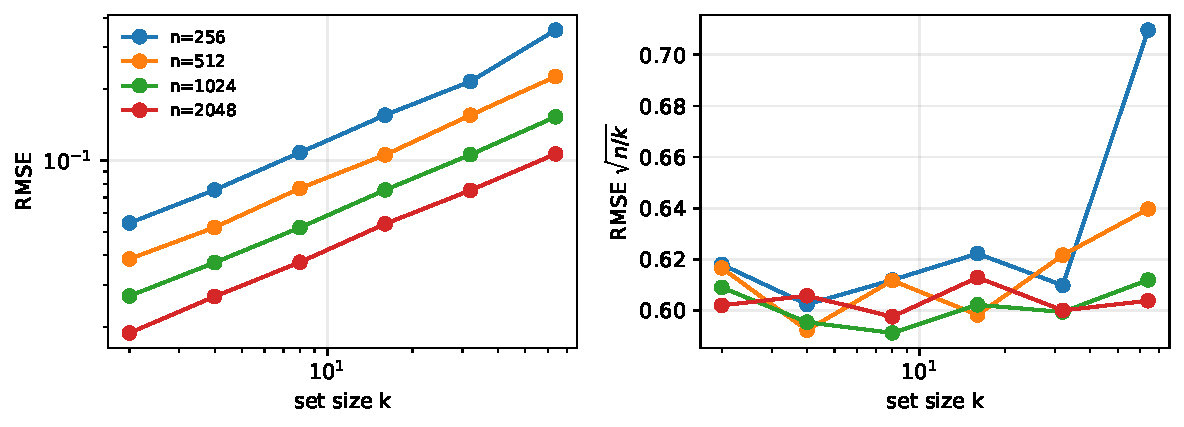
\includegraphics[width=\columnwidth]{scaling.pdf}
\caption{Balanced moment estimation under uniform cyclic attribution. The normalized RMSE is nearly constant.}
\label{fig:scaling}
\end{figure}

A positive-only score is badly biased because it retains the irrelevant feature mean. For example, at $(n,k)=(2048,64)$ its bias is $9.90$. Replacing the outside control by the global empirical feature mean appears close at small $k$, but is not exactly unbiased because the same source enters both the event count and the global mean. Its bias is $-0.0509$ at $(256,64)$ and follows the exact expression
\begin{equation}
 \frac{(1-\Sigma)(p\E g-\theta_g)}{n\Sigma}.
 \label{eq:globalbias}
\end{equation}
The balanced biases at $(256,64)$ and $(2048,64)$ are $0.0074$ and $-0.0003$, within Monte Carlo error. Code and all configuration-level results are included in the supplement.

\section{DISCUSSION}

The main lesson is that identifiability and statistical efficiency require different corrections. The earlier estimator identifies the risk for general attribution sets. Under translation, a second correction is available. Spreading negative mass outside each candidate set cancels nuisance fluctuations in both matrix coordinates. The remaining uncertainty is a canonical interaction whose energy is $n\Sigma$, not $n\Sigma^2$.

The upper and lower bounds settle the uniform worst-case dependence for stationary mechanisms. Three boundaries remain. Our upper theorem is finite-class rather than a full U-process result. The lower construction proves uniform sharpness across offset geometries but not geometry-by-geometry sharpness for consecutive windows. Finally, the path extension assumes a reporter-marked cohort. Removing that metadata while retaining exact boundary balance is open.

These limitations also point to useful next steps. Localized canonical U-process bounds could give fast rates under benign losses. Geometry-specific lower bounds could distinguish priors with the same $\ell_2$ norm. More broadly, balanced controls may apply whenever privacy mechanisms release translated candidate neighborhoods rather than individual links.

\bibliography{references}

\clearpage

\end{document}
